\documentclass[11pt]{article}
\usepackage[pdftex]{graphicx}
\usepackage[explicit]{titlesec}
\usepackage[OT1]{fontenc}
\usepackage[most]{tcolorbox}
\usepackage[final]{pdfpages}
\usepackage[colorlinks=true, urlcolor=cyan, hyperfootnotes=false]{hyperref}
\usepackage{fullpage, graphicx, psfrag, url, caption, authblk, amsfonts, amsmath, amssymb, float, fancyhdr, multicol, cmbright, xcolor, amsthm, gensymb, physics}

\fancypagestyle{pages}{
	%Headers
	\fancyhead[L]{Physics 7A, Summer 2024 \\ Section 103}
	%\fancyhead[C]{\thepage}
	\fancyhead[R]{Discussion 14 \\ July 24}
\renewcommand{\headrulewidth}{0pt}
	%Footers
	%\fancyfoot[L]{}
	\fancyfoot[C]{}
	\fancyfoot[R]{\thepage}
\renewcommand{\footrulewidth}{0pt}
}

\newcommand\blfootnote[1]{
    \begingroup
    \renewcommand\thefootnote{}\footnote{#1}
    \addtocounter{footnote}{-1}
    \endgroup
}

\newcommand{\fig}[4]{
    \begin{figure}[H]
        \centering
        \includegraphics[scale={#3}, angle={#4}]{#1}
        \caption{#2}
        \label{exp4fit}
    \end{figure}
}

\newtheoremstyle{gangnamstyle}{}{}{}{}{\sffamily\bfseries}{.}{ }{}
\tcolorboxenvironment{definition}{boxrule=0pt,boxsep=0pt,colback={blue!10},left=8pt,right=8pt,enhanced jigsaw, borderline west={2pt}{0pt}{blue},sharp corners,before skip=10pt,after skip=10pt,breakable}
\tcolorboxenvironment{example}{boxrule=0pt,boxsep=0pt,colback={orange!10},left=8pt,right=8pt,enhanced jigsaw, borderline west={2pt}{0pt}{orange},sharp corners,before skip=10pt,after skip=10pt,breakable}
\tcolorboxenvironment{problem}{boxrule=0pt,boxsep=0pt,colback={cyan!10},left=8pt,right=8pt,enhanced jigsaw, borderline west={2pt}{0pt}{cyan},sharp corners,before skip=10pt,after skip=10pt,breakable}
\theoremstyle{gangnamstyle}{\newtheorem{definition}{Definition}[]}
\theoremstyle{gangnamstyle}{\newtheorem{example}{Example}[]}
\theoremstyle{gangnamstyle}{\newtheorem{problem}{Problem}[]}

\headheight=0pt
\footskip=0pt
\setlength{\oddsidemargin}{0 in}
\setlength{\evensidemargin}{0 in}
\setlength{\topmargin}{-0.5 in}
\setlength{\textwidth}{6.5 in}
\setlength{\textheight}{8.5 in}
\setlength{\headsep}{0.75 in}
\setlength{\parindent}{0 in}
\setlength{\parskip}{0.1 in}

\begin{document}
\normalfont
\pagestyle{pages}

% Begin Document

\begin{center}
\vspace{3in}
{\Large Discussion 14 } \\ [0.05in]
Midterm Review \\ [-0.5in]
\end{center}

\section{Review}

I was made aware that some of you may find these gravitation problems helpful. 

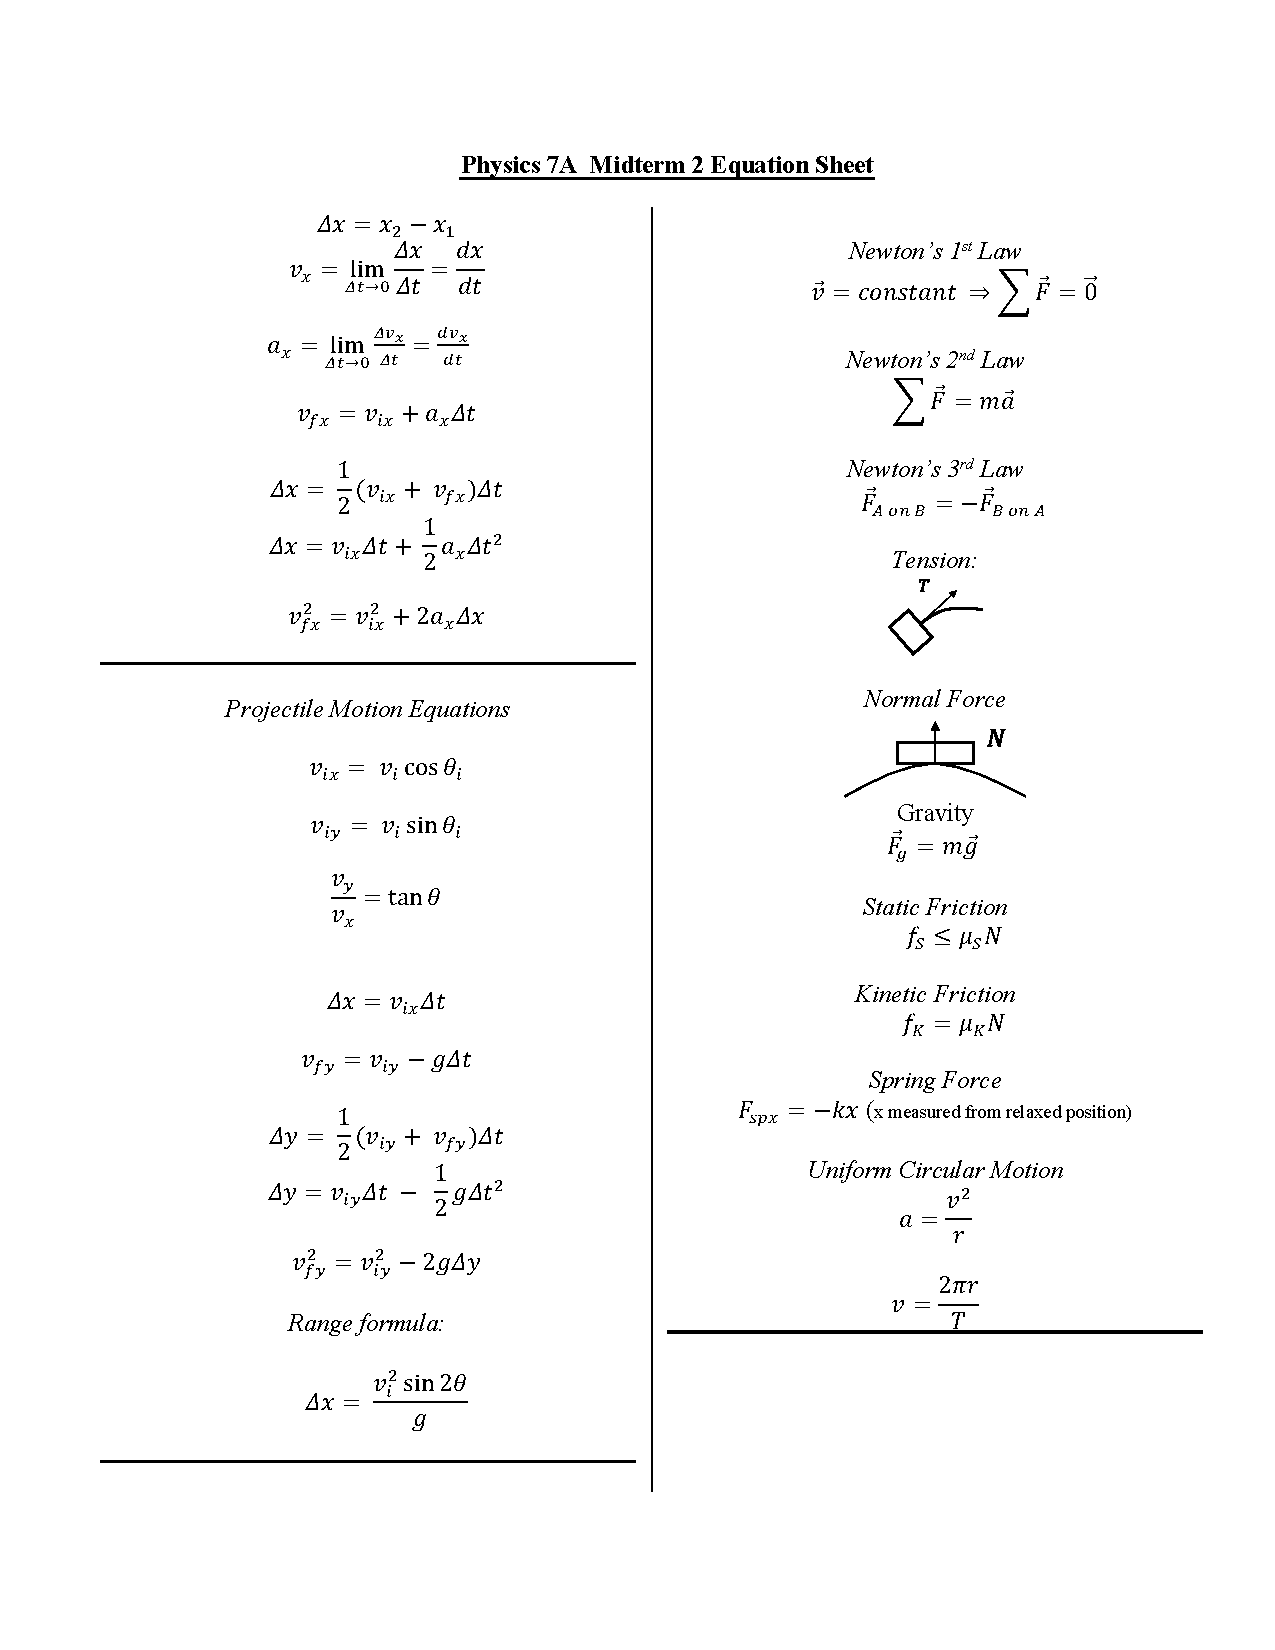
\includepdf[pages=-]{figs/mt2/equation.pdf}

\textbf{1.} \textit{Physics 7A Past Exam Problem} \\
The force of gravity for two masses $M$ and $m$ can be written:
\[ \Vec{F} = \frac{-GMm}{r^2} \hat{r} \]
where $r = 0$ is the center of mass of $M$ and $\hat{r}$ points in the direction of $m$ (that is, gravity is an attractive force).

a) Derive the potential energy of this force and make a sketch of this function. Explain any choices you made in defining the potential energy. 

b) Derive an expression for the “escape velocity” needed to fully escape the earth’s gravity starting from the surface of the earth, $r = R_E$. 

c) Now consider a satellite in circular orbit around the earth. The Virial Theorem says that the average kinetic energy is equal to $1/2$ the absolute value of the potential energy for many systems. Is it true for the orbiting satellite? 

\pagebreak

\begin{center}
(Blank Page)
\end{center}

\pagebreak

\textbf{2.} \textit{Physics 7A Past Exam Problem} \\
A lunar lander is approaching the Moon along a low-altitude parabolic trajectory. At the point of closest approach to the Moon, the lander was barely scraping off the surface of the moon. At this radius, the mission control briefly turns on the braking engine, so that the lander starts to execute a circular orbit about the moon. Determine the change in the lander’s velocity during the maneuver. 

Mass of the Moon: $M = 7.4 \times 10^{22} \ kg$. 

Radius of the Moon: $R = 1.7 \times 10^{6} \ m$. 

Gravitational Constant: $G = 6.67 \times 10^{-11} \ m^3/kgs^2$. 

\pagebreak

\begin{center}
(Blank Page)
\end{center}

\pagebreak

\textbf{3.} \textit{Physics 7A Past Exam Problem} \\
A more precise form of the potential energy of a planet with mass $m$, orbiting the sun (mass $M$) at a distance $r$ is:
\[ U(r) = \frac{-GMm}{r} + \frac{L^2}{2mr^2} \]
Where $L$, the magnitude of angular momentum, is a constant. 

a) Determine the stable equilibrium radius, $r_{eq}$, where the planet would feel no radial force from the sun. Find $U(r_{eq})$, the potential energy at the equilibrium position. 

b) Sketch the general form of $U(r)$. You do not need to be precise, but the graph should capture any asymptotic behaviors or the rough locations of local minima and maxima. 

c) For an object with total energy $E = \frac{1}{2}U(r_{eq})$, what are its turning points? 

\pagebreak

\begin{center}
(Blank Page)
\end{center}

\pagebreak

\textbf{4.} \textit{Physics 7A Past Exam Problem} \\
A sudden impulse $J$ is applied to a billiard ball of mass $m$ and radius $r$ at a spot $0.4r$ below the ball’s center. Assume $J$ acts over a very short time.

\fig{figs/mt2/tbp5.png}{Impulse and Collision}{0.65}{0}

a) Find the translational and rotational velocity of the ball just after the impulse is applied.

b) The ball immediately collides elastically with a second billiard ball (same mass and radius) that is at rest. Find the translational and rotational velocities for both balls just after the collision. The collision occurs in a very short time, and there is no friction between the balls.

c) The coefficient of kinetic friction between the balls and the table is $\mu_k$. Solve for the translational and rotational motion of both balls as a function of time after the collision.

d) Is total mechanical energy conserved? Explain your reasoning and provide quantitative proof.

\pagebreak

\begin{center}
(Blank Page)
\end{center}

\pagebreak

\end{document}
